\documentclass[12pt]{article}
\usepackage[margin=1in]{geometry}
\usepackage{graphicx}
\graphicspath{ {images/} }
\usepackage{fontspec}
\setmainfont[Path=/usr/share/fonts/truetype/calibri/,
    BoldItalicFont=CALIBRIZ.ttf,
    BoldFont      =CALIBRIB.ttf,
    ItalicFont    =CALIBRII.ttf]{Calibri.ttf}
\title{Lab 07: Torque, Equilibrium and Center of Gravity: Balancing}
\author{Adris Jautakas, partnered with Matthew Kendall}
\date{January 22, 2018}
\begin{document}
    \maketitle
    \pagebreak
    \section*{Abstract}
        \begin{quote}
        {\textit {\small 
            In this lab, the physics of rotational static equilibrium were 
            explored and evaluated with a meter stick scale. We proved the
            laws describing rotational equilibrium through multiple methods
            of balancing and adjusting the scale. By verifying these mechanics,
            we can understand how they are utilized in the real world.
        } }
        \end{quote}

    \section{Introduction}
        In our experiment, the concept of static equilibrium was explored
        with a balancing rod. Static equilibriums involve balancing out the
        forces of a system to cancel out all acceleration. In this case, we are
        focusing on a rotational static equilibrium where the net torque of the
        system cancels the rotational acceleration of the rod. The torque and
        angular acceleration of a rod can be determined with physical laws, and
        in this experiment we emperically find the torques required to form a
        static rotational equilibrium to determine the accuracy of these laws.

    \section{Materials}
        \begin{itemize}
            \item Meterstick
            \item Stand
            \item Hinge clip that can attach to meterstick and rotate around the 
                  stand
            \item Set of weights, including an unknown mass
            \item String and clips that can attach the weights to the meterstick
        \end{itemize}
    
    \section{Methods}
        \subsection{Experiment Setup}
            The experiment is set up by fixating the stand perpendicular to the
            ground and attaching the meterstick to the stand via the hinge clip.
            For each experiment, attach a mass at a specified distance from the
            pivot point. For the first set of experiments, the meterstick should
            be attached at its center of mass (right down the middle) and masses
            and another mass's position will be adjusted to reach equilibrium.
            For the second set of experiments, the attachment point will be 
            adjusted to reach equilibrium

    \section{Data}
        {\large Experiment 1: Apparatus with Point of Support at Center of Gravity} \\
        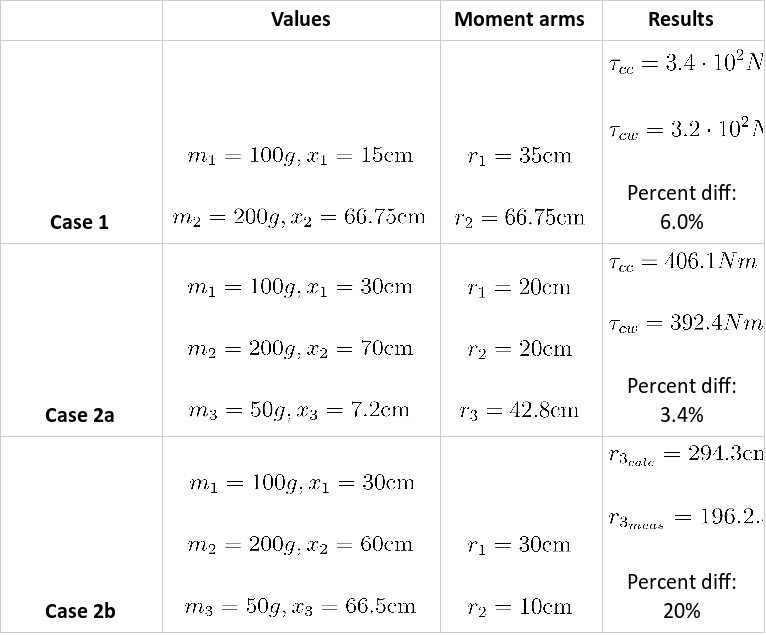
\includegraphics[scale=0.5 ]{Table1.png} \\ \\
        \begin{minipage}{\linewidth} % Keeps it together without breaking
            {\large Experiment 2: Apparatus Supported at Different Pivot Points} \\
            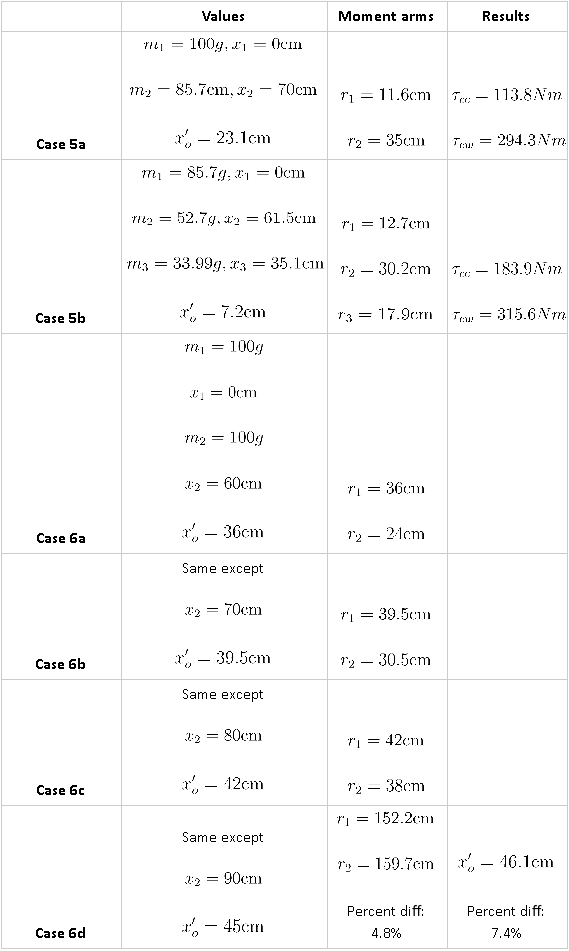
\includegraphics[scale=0.7 ]{Table2.png} \\ \\
        \end{minipage}
    \section{Analysis}
        \subsection{Equations}
            In a system, linear and rotational equilibrium are acheived when
            the net force and net torque are zero, respectively. This can be
            expressed as
            \begin{equation}
                \sum F_i = 0
            \end{equation}
            \begin{equation}
                \sum T_i = 0
            \end{equation}
            In this example, we do not need to worry about linear equilibrium
            because the tension of the string on the meterstick cancels out the
            force of gravity of the weights. Tension is defined with the
            equation $\vec{T} = \vec{r} \times \vec{F}$ where $\vec{T}$ is tension, 
            $\vec{r}$ is the distance from the center of rotation and $\vec{F}$
            is the force applied at that point. Since we assume that $\vec{r}$
            and $\vec{F}$ are perpendicular to each other, we simplify this
            equation to $T = rF$. The only force acting on each block is their
            force of gravity. Knowing all of this, we rewrite our equation as
            \begin{equation}
                \sum r_im_ig = 0
            \end{equation}
            When we find the equilibrium of a system, we can check the masses
            and their radii from the pivot point to determine whether they
            accurately reflect the laws described above.
    
    \section{Conclusion}
        Although our percent error fluctuated a little bit, maxing out at a
        whole 20\% for one experiment, for the most part it was relatively low.
        This error can be caused by a number of factors, including the friction
        between the axle and the meter stick.
        This can confirm that the equations describing torque are accurate in
        the real world.
\end{document}
